\documentclass[11pt]{scrartcl}

\usepackage[sexy]{evan}
\usepackage{pgfplots}
\pgfplotsset{compat=1.15}
\usepackage{mathrsfs}
\usetikzlibrary{arrows}
\usepackage{graphics}
\usepackage{tikz}
\usepackage{ amssymb }
\usepackage[dvipsnames]{xcolor}
\usepackage[utf8]{inputenc}
\usepackage{longtable}
\usepackage{ragged2e}
\usepackage{listings}


\definecolor{noseve}{RGB}{242,242,242}

\newcommand{\camod}[1]{\frac{\ZZ}{#1 \ZZ}}
\newcommand{\modm}[1]{\text{ mod } #1}
\newcommand{\campm}[1]{\frac{\ZZ}{m\ZZ}}

\usepackage{epigraph}
\renewcommand{\epigraphsize}{\scriptsize}
\renewcommand{\epigraphwidth}{60ex}


\definecolor{dcol0}{HTML}{C8E6C9}
\definecolor{dcol1}{HTML}{D4E9B3}
\definecolor{dcol2}{HTML}{E5ED9A}
\definecolor{dcol3}{HTML}{FFF59D}
\definecolor{dcol4}{HTML}{FFE082}
\definecolor{dcol5}{HTML}{FFCC80}
\definecolor{dcol6}{HTML}{FFAB91}
\definecolor{dcol7}{HTML}{F49890}
\definecolor{dcol8}{HTML}{E57373}
\definecolor{dcol9}{HTML}{D32F2F}

\makeatletter
\newcommand{\getcolorname}[1]{dcol#1}
\makeatother

\newcommand{\dif}[1]{%
    \edef\colorindex{\number\fpeval{floor(#1)}}%
    \edef\fulltext{#1}%
    \colorbox{\getcolorname{\colorindex}}{%
        \ifnum\colorindex>8
            \textbf{\textcolor{white}{\,\fulltext\,}}%
        \else
            \textbf{\textcolor{black}{\,\fulltext\,}}%
        \fi
    }%
}
% Variable para dificultad (inicial 0)
\newcommand{\thmdifficulty}{0}

% Comando para asignar dificultad antes del problema
\newcommand{\problemdiff}[1]{\renewcommand{\thmdifficulty}{#1}}

% Estilo del problema que incluye dificultad antes del título
\declaretheoremstyle[
    headfont=\color{blue!40!black}\normalfont\bfseries,
    headformat={%
      \dif{\thmdifficulty}\quad \NAME~\NUMBER\ifx\relax\EMPTY\relax\else\ \NOTE\fi
    },
    postheadspace=1em,
    spaceabove=8pt,
    spacebelow=8pt,
    bodyfont=\normalfont
]{problemstyle}

    \declaretheorem[style=problemstyle,name=Problema,sibling=theorem]{problema}
    \declaretheorem[style=problemstyle,name=Problema,numbered=no]{problema*}

%\usepackage[
%backend=biber,
%style=alphabetic,
%sorting=ynt
%]{biblatex}
%\addbibresource{referencias.bib}

\newcommand{\indicacion}[1]{\noindent\textit{\small #1}}


\title {Practica 5: Practica de comunicación serial}
\subtitle{Unidad II: Interfaces de comunicación Tema 2.1 \\ Sistemas Embebidos II 18MPEDS0729 \\ Ago-Dic 2025 \\ Centro de Enseñanza Tecnica Industrial Plantel Colomos\\Tgo. en Desarrollo de Software \\ Academia: Sistemas Digitales \\Profesor: Antonio Lozano Gonzáles }
\date{19 de Octubre de 2025}
\author{Emmanuel Buenrostro 22300891 7F1 \\ \and Emiliano Arzate 22300929 7F1 \\}


\begin{document}

\maketitle
\begin{center}
   
\includegraphics[scale=0.15]{../../cetilogo.jpg} 
\end{center}
\newpage

\section{Objetivo}
 Enviar y recibir información serial utilizando solo dos cables o alambres, para reducir peso y costo en las instalaciones.
\section{Desarrollo de la Práctica}

\subsection{Condiciones de la Práctica}
Utilizando su arduino, deberán establecer comunicación serial con otro equipo. Dicha comunicación serial sera Ful Duplex. es decir, transmitirá y recibirá información al mismo tiempo. Lo que se deberá enviar y recibir serán caracteres y números, todos los caracteres de  nuestro idioma español, ya sea en mayúsculas o minúsculas, también los números del 0 al 9. Para enviar dicha información se utilizara el teclado hexadecimal y una pantalla LCD, en los dos equipos arduino. 
Recuerde que los dos equipos trasmitirán y recibirán la información.

\subsection{Algoritmo o Diagrama de Flujo}

\begin{enumerate}
  \item Inicializaciones: configurar LCD, keypad y la cadena global \texttt{s}.
  \item setup(): iniciar \texttt{Serial}, \texttt{Serial3} y el LCD.
  \item loop(): obtener número con \texttt{readnumber()} y enviarlo por \texttt{Serial} y \texttt{Serial3}.
  \item readnumber(): en bucle leer teclas y \texttt{Serial3}; acumular dígitos en un entero; terminar al presionar '\*'.
  \item leerSerial(): si hay datos en \texttt{Serial3} concatenarlos a \texttt{s} y llamar a \texttt{imprimir()}.
  \item imprimir(): limpiar LCD y mostrar \texttt{s}.
\end{enumerate}

\subsection{ Código C}

\lstinputlisting[language=C]{Pr5/Pr5.ino}


\section{Observaciones y Conclusiones}

\begin{itemize}
    \item Usamos distintos seriales, ya que el Serial1 es el que esta usando la computadora, para conectar los arduinos usamos el Serial3.
    \item Ahora tuvimos que hacer un teclado que lea por ASCII mas que solo lo del teclado.
\end{itemize}
  

\section{Imagen}

\begin{center}
    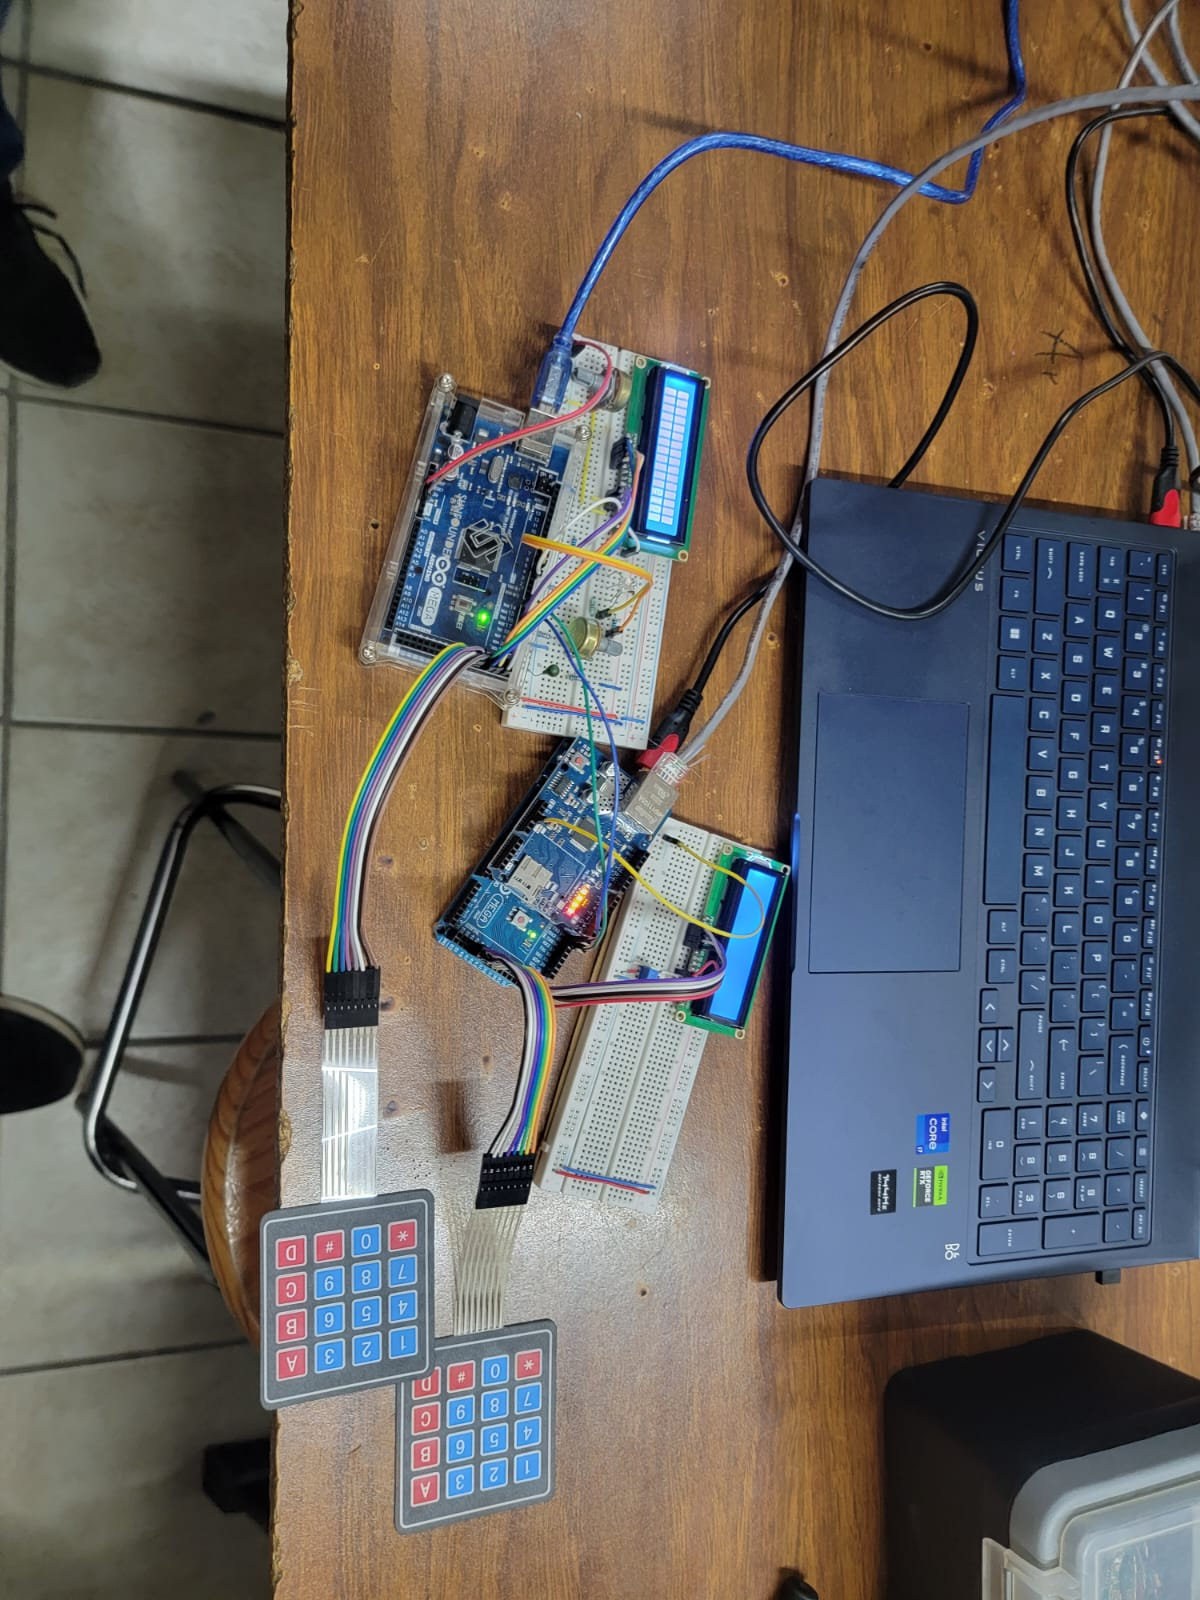
\includegraphics[scale=0.3]{imagen_circuito.jpg}
\end{center}
%\nocite{*}

%\printbibliography[
%heading=bibintoc,
%title={ . }
%]
    \end{document}